\documentclass[a4paper,11pt]{report}
%
%--------------------   start of the 'preamble'
%
\usepackage{graphicx,amssymb,amstext,amsmath}
\usepackage{listings}
\lstset{postbreak=\space, breakindent=2pt, breaklines, basicstyle=\scriptsize, tabsize=4}

%
%%    homebrew commands -- to save typing
\newcommand\etc{\textsl{etc}}
\newcommand\eg{\textsl{eg.}\ }
\newcommand\etal{\textsl{et al.}}
\newcommand\Quote[1]{\lq\textsl{#1}\rq}
\newcommand\fr[2]{{\textstyle\frac{#1}{#2}}}
\newcommand\miktex{\textsl{MikTeX}}
\newcommand\comp{\textsl{The Companion}}
\newcommand\nss{\textsl{Not so Short}}
%
%---------------------   end of the 'preamble'
%
\begin{document}
%-----------------------------------------------------------
\title{Cuda-Keccak}
\author{Giuseppe Chindemi, Nicola Crovetti}
\maketitle
%-----------------------------------------------------------
\begin{abstract}\centering
The abstract \dots
\end{abstract}
%-----------------------------------------------------------
\tableofcontents
\newpage
\listoffigures
%-----------------------------------------------------------
\chapter{Introduction}
\dots\\

\chapter{Keccak Overview} \label{chap:keccak-overview} 
Keccak is a family of hash functions that are based on the sponge construction and use as a building block a permutation from a set of 7 permutations.
In this overview, we specify these permutations and the Keccak sponge functions. For more information, and for the reference code, please refer to the Keccak web page.

\section{The Keccak-f permutations}
There are 7 Keccak-f permutations, indicated by Keccak-f[b], where \({b = 25 \times 2^l}\) and
l ranges from 0 to 6. Keccak-f [b] is a permutation over \({s \in Z^b_2}\), where the bits of s are 
numbered from 0 to \({b − 1}\). We call b the width of the permutation.\\

In the sequel, the permutation Keccak-f[b] is described on a state \({a}\) that is a three-dimensional array of elements, namely \({a[5][5][w]}s\), 
with \({w = 2l}\). The mapping between the bits of \({s}\) and those of \({a}\) is \({s[w(5y + x) + z] = a[x][y][z]}\). The expression \({a[x][y][z]}\) with
\({x, y \in Z5}\) and \({z \in Z_w}\) , denotes the bit in position \({(x, y, z)}\). It follows that indexing starts from
zero; expressions in the x and y coordinates should be taken modulo 5 and expressions in the
\({z}\) coordinate modulo \({w}\). Both the [y][z] indices or all
three indices, implying that the statement is valid for all values of the omitted indices.\\

Keccak-f [b] is an iterated permutation, consisting of a sequence of \({nr}\) rounds \({R}\), indexed
with \({i_r}\) from 0 to \({nr − 1}\). A round consists of five steps:\\


	$R = \iota \circ \chi \circ \pi \circ \rho \circ \omega$ ,   with \\


\({	\omega : a[x][y][z] \leftarrow a[x][y][z] + \sum_{y'=0}^4 a[x − 1][y'][z] + \sum_{y'=0}^4 a[x + 1][y ′ ][z − 1] ,} \)\\

$\rho : a[x][y][z] \leftarrow a[x][y][z − (t + 1)(t + 2)/2]$,\\
with t satisfying 0 $\leq$ t $<$ 24 and
$ \left( \begin{array}{cc}
0 & 1 \\
2 & 3 \\
\end{array}
\right)^{t}
\left(
\begin{array}{c}
1 \\
0 \\
\end{array}
\right) =
\left(
\begin{array}{c}
x\\
y\\
\end{array}
\right)
$ in GF$(5)^{2 \times 2}$,\\
or $t = -1$ if $x = y = 0$ \\

$ \pi: a[x][y] \leftarrow a[x'][y'] $, with
$\left( \begin{array}{c}
x \\
y \\
\end{array}
\right) = \left( \begin{array}{cc}
0 & 1 \\
2 & 3 \\
\end{array}
\right)
\left( \begin{array}{c}
x' \\
y' \\
\end{array}
\right)$\\

$\chi: a[x] \leftarrow a[x] + (a[]x+1]+1)a[]x+2$\\

$\iota: a \leftarrow a + RC[i_r]$ \\


The additions and multiplications between the terms are in GF(2). With the exception of
the value of the round constants $RC[i_r]$, these rounds are identical. The round constants are
given by (with the first index denoting the round number)\\

$RC[i_r][0][0][2^j − 1] = rc[j + 7i_r ]$, for all $0 \leq j \leq l$,\\

and all other values of $RC[i_r][x][y][z]$ are zero. The values $rc[t] \in $ GF(2) are defined as the
output of a binary linear feedback shift register (LFSR):\\

$rc[t] = (x^t$ mod $x^8 + x^6 + x^5 + x^4 + 1)$ mod $x$ in GF(2)[x].\\

The number of rounds nr is determined by the width of the permutation, namely,\\

$n_r = 12 + 2l$



\chapter{CUDA Overview} \label{chap:cuda-overview}
CUDA is a software layer that allow programmers to exploit the capability of nVidia GPUs as general purpose processors.\\
Dealing with a video card in this way requires approaching a completely new programming style and acquiring some knowledge about the basic nVidia GPUs architectures, even though all the internal details are masked by the framework.\\
First of all, as a philosophical remark, a GPU cannot run anything conceived and written for a CPU, as every vector stream architecture. In order to product software that can be executed on a CUDA Capable GPU, the programmer must write natively parallel code using one of the supported languages, extended with ad hoc CUDA primitives. There is no tool that can perform automatic porting of a sequential code into a parallel one.\\
CUDA exposes the GPU as a "Parallel Co-Processor" that can be used by the CPU to speed-up the computations. More in the details, the CPU - Host - can take advantage of the high amount of parallel threads executable by the GPU - Device - to accelerate parts of a program that are especially well suited for exploiting TLP. According to this approach, the CPU must directly manage the program execution settings on the GPU, provide the data for the computation to the device and collect the outputs when it is done.\\
One of the most important features of CUDA is that it abstracts away all the physical details of the supported GPUs and always shows to the programmer  the very same logical organization (Figure \ref{fig:nVidiaGPUsLogicalOrg}). These GPUs can be considered a MIMD array of SIMD processors, called MultiProcessors. Each MultiProcessor is composed of 3 elements: a fixed number of cores, an instruction unit and a private memory space. All the MultiProcessors share a pubblic memory space referred to as Device Memory in order to distinguish it from the CPU memory space - Host Memory - that is not directly accessed by the GPU. Due to the property of abstraction mentioned before, the only difference between families of nVidia products is in the amount of memory, the number of MultiProcessor and the nature of the cores.\\
These factors divide CUDA GPUs into subfamilies identified by an ID, the so called 'Compute Capability'. Some advanced CUDA primitives and features requires a specific Compute Capability.\\  
\begin{figure}[h!bt]
	\centerline{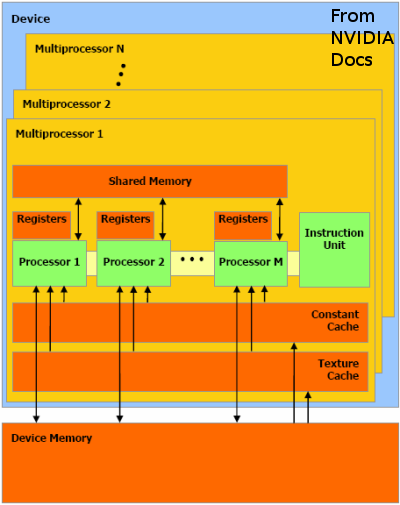
\includegraphics[width=0.5\textwidth]{img/hw-model.png}}
	\caption{Logical Organization of all the CUDA capable devices. The programmer does not have to take care of the physical organization of the GPU that will actually execute the program.}
	\label{fig:nVidiaGPUsLogicalOrg}
\end{figure}
\section{Multiprocessors}
Even if the architectural details of the CUDA capable GPU can significantly differ from a product to another, some common guidelines can be identified.\\
As stated before the MP is a SIMD component: all the SPs belonging to the same MP execute the same instruction on different data. This structure, obviously deigned for graphical purpouses, make the GPUs also particulary effective in addressing problems that can exploit a huge amount of TLP.\\
Form a philosophical point of view, the MPs of these GPUs are designed to be as simple and fast as possible. In order to keep low the complexity, there are neither branch predictors, nor mechanisms to rollback incorrect results. Even if this seems a serious limitation to the performance, it allow the cores of the MP to be completely focused on the arithmetic intensity. As results of this choice, the SPs of the most recent nVidia products are able to perform a double precision MAD (or MUL or ADD) per clock cycle.\\

\section{Memory Hierarchy}
The CUDA memory hierarchy consists of several elements optimized for different memory usages.\\
The Device Memory is the main memory space of the GPU. It can be accessed by both the CPU and the GPU using different policies, usually with a latency of some hundreds of clock cycles. In order improve the performance and the usability, it is logically partitioned into three logic component, depending on the access method: the Global Memory, that follow the common 32-,64-, or 128-byte memory transactions paradigm; Texture Memory, accessed by texture fetching; Constant Memory, managed by special operations.\\
The Global Memory is the most frequently employed memory space. Usually it is used by the CPU to load the data for the computations into the device and by the GPU to provide the results. Furthermore the Global Memory is the only space completely shared among all the SPs of the device: for this reason it is also exploited for comunication among SPs belonging to different MPs. Part of the Global Memory can be used, if necessary, to extend the private memory space of each SP. This special region of the Global Memory is called Local Memory. The Texture Memory can be written by the CPU using the CUDA API and readed by the GPU via texture fetching. No GPU texture write mechanism is provided. The Constant memory is a small special memory space that can be used for allocation of variables frequently readed. These variables must be allocated by the CPU before the execution on GPU, that can access them solely in read-only mode.\\ 
Due to the high latency of the Device Memory, each MP is provided with a private low latency memory space, logically divided into:
\begin{itemize}
\item a so called Shared Memory, directly accessible by all the SPs of the MP
\item a Constant Cache and a Texture Cache, managed by the framework
\item a set of exclusive Registers for each SP
\end{itemize}
The Shared Memory can be considered as both a sort of "cache" of the Global Memory 
 directly administrated by the cores in the MP and a mechanism for communicating among SPs belonging to the same MP. The Constant Cache and the Texture Cache are L1 caches used to speed-up the access time of the Constant Memory and the Texture Memory, respectively. Due to the fact that Constant Memory and Texture Memory are read-only (from a GPU point of view), no cache coherency protocol is required.\\ 

\section{Programming Model}
As stated at the beginning of this chapter, the CUDA framework enable the programmer to take advantage of the high number of parallel threads executable by the GPU to expoit TLP: ideally the program is organized into identical sub-problems - working on different data - that can be solved independently. Each of this sub-problems, called Kernels, is mapped onto a thread that will be executed on a SP.\\
All the threads executed by the SPs of a single MP are logically organized into a structure called Block. Virtually speaking, all the Threads belonging to a Block are execuded in parallel. Usually, the number of SPs in a MP is much less than the number of Threads in a Block. For this reason, only a subpart of the Threads is in concurrent execution at a given time - the so called Warp. When a MP is loaded with a Block, it partitions it into warps that get sheduled by a warp sheduler for the execution on that MP. Due to the fact that all the Threads of a Block are executed on the same MP, it should be noticed that they share all the MP resources (i.e. Shared Memory and Caches) and that they can be synchronized using a specific API barriers.\\
All the Blocks are grouped into another logical structure called Grid. Considering that the number of Blocks of the Grid is usually greater than the number of MPs, not all the Blocks can typically be sheduled at the same time. Since the blocks are unordered, they can execute equally well on a GPU that can handle one block at a time and on one that executes a dozen or a hundred at a time, as a demonstration of the scalability offered by the framework. In order to avoid complicating the Block scheduling process, no extra-block threads syncronization mechanism is provided.\\ 

\begin{figure}[h!bt]
	\centerline{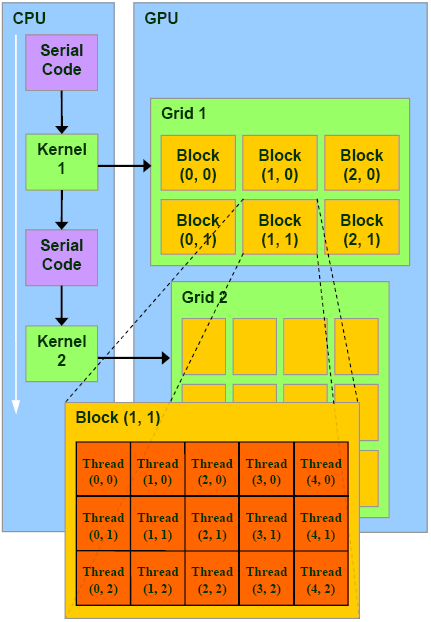
\includegraphics[width=0.5\textwidth]{img/nvidia-execution-model.png}}
	\caption{nVidia Execution Model, an example of heterogeneous programming.}
	\label{fig:nvidia-exec-mod}
\end{figure}

\section{Best Practices}
In order to best exploit the resources of a CUDA capable GPU, there are several practices that must be adopted. Even if many of these are strictly dependent on the specific device used, there are some general rules that can be easily identified:
\begin{description}
\item[Memory Transfers] between Host and Device must be reduced to the minimum. Ideally there should be only one transfer Host-Device to store on the GPU the data for the computation and one transfer Device-Host to collect the results.
\item[GPU Occupancy] must be maximized. That is, the number of warps actually in execution must be closer to the maximum number of "in-fly" warps supported by the Device.
\item[Divergent Branches] should be avoided. Due to the fact that all the threads of the warp must execute the same instruction, in case of divergent branches the warp execution will be serialized, reducing the performance.
\item[Local Memory] usage should be limited in favor of registers because of the high latency of the former.  
\item[Compute Capability] must be considered in order to both tune the GPU execution parameters and avoid unsupported operations.
\end{description}
These three good pratices, ordered by decreasing importance, could be considered the most important rules that must be observed to effectivly developing in CUDA. It should be noticed that in the past this list was expanded by at least one element, coalescence. In the first CUDA Devices - identified by a so called "compute capability" berween 1.0 and 1.1 - all the threads in the same warp had to access the memory words in sequence and, consequently, to avoid multiple reads/writes. Only if this pratice is enforced the MP can reduce to the least the number of memory accesses needed to provide the data to all the SPs. With modern devices - compute capability grater or equal to 1.2 - this constraint is much more relaxed: threads can access any word in any order, including the same words, and a single memory transaction for each segment addressed by the warp is issued. In this cases the problem of coalescence can be completely forgotten.

\chapter{Design}\label{chap:design}
In this Chapter the two approach to the parallelization of Keccak will be presented. As stated in Chap. \ref{chap:introduction}, the solutions proposed try to reduce the time needed to the hash computation by addressing the problem in two diametrically opposed ways: the first solution, from now on referred to as "local parallelization", attempts to increase the time performance by means of a bunch of threads collaborating for the computation of a single hash; the second solution, from now on referred to as "global parallelization", concentrates on the simultaneous calculation of the hash of different messages, taking advantage from the consideration that usually in the real world the software for the computation of the hash is installed on machines that must serve thousand of different requests per second.\\
In the following sections the two approaches will be extensively presented.\\


\section{Local Parallelization}
The internal status of the Keccak permutation function is composed by 25 words of 64 bits in a grid 5x5. Since in CUDA the bit to bit operations are rather slow, we decided to use 25 thread, one for every word of the internal state. As described below, every single thread, during the computation, is responsible for calculating the value of a single cell of the matrix, identified by the positions X and Y of the state matrix that are the same of thread in the CUDA thread-grid.

\subsection{Chi}
In the implementation of chi we used a matrix 10x5 of 64 bits words, containing the internal state of the Hash function after the previous step, replicated two times. This because, in CUDA, the modulo operator is rather slow compared with cpu; using a 10x5 matrix the threads that need words out of the first 5 columns of the matrix can safety complete the operations. The operators NOT, XOR and AND have been used normally. The result is written in a new matrix that will be the new internal state.

\subsection{Theta}
In the implementation of Theta the internal state is duplicated in a matrix 5x10 for the same reason described for Chi. Every single thread calculate the C value of its own column so that it is repeated 5 times (one for every thread of the column). This procedure is aimed to avoid using IF-patterns that would break the parallelism between thread. The D matrix is calculated in the same way. For the computation of the ROT matrix we were forced to use shift operators that can decrement the performance. At the end every thread copy its result in the corresponding cell of a new matrix that will be the new internal state.

\subsection{Pi}
The Pi step is implemented using 2 matrix 5x5 with the coordinates X and Y of the new positions that the words will have after the permutation. Every thread read this coordinates and copy its state word in a new matrix, in the position read, that will be the new internal state.

\subsection{Rho}
Like in the Theta, in Rho we were forced to used shift operators to implement the bit word rotation; the offset of the rotation depends on the position of the word to rotate in the internal state and is loaded as constant in a 5x5 matrix. The single thread read the offset value and make the rotation of its own word and then copies the result in a new matrix.

\subsection{Iota}
The implementation of Iota is obviously the more simple since in Iota there is only a bit to bit xor between the first word of the internal state and a 64 bits constant different in every round. Those round constant are preloaded and the operators has been used normally.


\section{Global Parallelization}
The original Keccak structure have been almost completely maintained in this solution, even thought many adjustments have been made to maximize the performance on GPU. This optimization process required the main effort: the tuning of both the execution parameters and the compiler directives leads to the production of very different algorithms before the best configuration has been discovered.\\
Following a description of the base algorithm and a discussion of the most important design choices.\\

\subsection{Base Algorithm}
All the designed algorithms have a common base, showed in Alg. \ref{alg:cuda-keccak}
\begin{algorithm}                      % enter the algorithm environment
\caption{Calculate $y = x^n$}          % give the algorithm a caption
\label{alg:cuda-keccak}                % and a label for \ref{} commands later in the document
\begin{algorithmic}                    % enter the algorithmic environment
\REQUIRE $n \geq 0 \vee x \neq 0$
\ENSURE $y = x^n$
\STATE $y \Leftarrow 1$
\IF{$n < 0$}
\STATE $X \Leftarrow 1 / x$
\STATE $N \Leftarrow -n$
\ELSE
\STATE $X \Leftarrow x$
\STATE $N \Leftarrow n$
\ENDIF
\WHILE{$N \neq 0$}
\IF{$N$ is even}
\STATE $X \Leftarrow X \times X$
\STATE $N \Leftarrow N / 2$
\ELSE[$N$ is odd]
\STATE $y \Leftarrow y \times X$
\STATE $N \Leftarrow N - 1$
\ENDIF
\ENDWHILE
\end{algorithmic}
\end{algorithm}
The only difference between all the solutions designed is the kernel adopted for the computations. Three different kernels have been produced:\\
\begin{itemize}
\item \textbf{Kernel Base} Almost identical to the Keccak reference permutation function.
\item \textbf{Kernel Unrolled} All the loop have been unrolled in order to avoid thr continuous flush of the computation pipeline.
\item \textbf{Kernel SH} Local variable have been placed into shared memory to prevent the usage of the slow Local Memory.
\end{itemize}
The test performed showed that 'Kernel Unrolled' is the most effective. Further details on this in Chap. \ref{chap:conclusions}.

\subsection{Memory Transfers}
Memory transfers between Host and Device Memory are the main cause of performance lost in the CUDA applications.\\
In this work, from the logical point of view, there is a need for a single large data transfers from the Host to the Device: the messages by which to evaluate the hashes. The retrieval of the computed hashes can be considered negligible compared to the previous data flow. The most obvious solution to provide the data for the computations to the GPU is of course a single big data transfers from the Host, however, this idea has been rejected because judged unnecessarily onerous. This assertion emerges from the consideration that only one token of each message can be considered at a time, because of the serial nature of Keccak. For this reason the data flow has been partitioned into tokes and performed using a double buffer strategy: during the computations of the \textit{i th} token, the data needed for the \textit{i+1 th} one are loaded into a separate memory location. It has been verified that the latency of these memory transfers is completely hidden by the kernel execution.

\subsection{Loop Unrolling}
As mentioned in Chap. \ref{chap:cuda-overview}, no branch prediction strategy is implemented into CUDA devices. For this reason loops can be a source of trouble in CUDA applications, especially if they are many and consist of a few instructions, as in this case.\\
Considering that the nvcc compiler has often an unpredictable behaviour and that it is still an open highly variable project, the loops founded in the original code have been physically fully unrolled instead of using the compiler unroll directive. The results obtained by this operation were satisfying and have influenced the choice of the unrolled kernel as reference version for the project.

\subsection{Registers Usage}
Registers usage is a sore point for all the CUDA applications. These are the default location of local variables and contain temporary results of arithmetic operations.\\
In order to maximize the occupancy, and consequently the performance, the number of used registers per thread must be kept under very limited thresholds, depending on the compute capability of the device. On the other hand, registers are the fastest memory locations available in the GPU and for this reason their usage is strongly encouraged, still for the performance implications.\\
The nvcc compiler by default attempt to maximize the registers usage. Unfortunately, when the total amount of memory requested by a thread exceed the registers availability, the compiler can decide to place local variables and temporary result into a special part of the Global Memory, the so called Local Memory. This locations are private and have the scope of a single threads like registers, but unlike registers these are located off-chip and have the same high latency of the Global Memory. For this reason the usage of Local Memory must be avoided.\\
This work, by its own nature, is highly registers intensive and for this reason suffers from limited availability of fast memory: a big part of the local variables of the threads are allocated into Local Memory. In order to reduce the impact on performance, a special kernel that uses the shared memory as local variables location has been designed.

\subsection{Left Shift}
A well-known nvcc bug has been a source of problems in the early stages of development. The bug, reported to the nvidia community a long time ago but not yet corrected, concerns to the inability of performing bitwise left shift when the shift factor is not stored into a constant variable. As suggested by nvidia itself, in order to bypass the problem the shift factor have been copied into a constant variable immediately before the shift operations.

\chapter{Results} \label{chap:results}
\section{Local Parallelization}
\section{Global Parallelization}



\chapter{Conclusions} \label{chap:conclusions}
The 'sigle implementation' of CUDA Keccak did not achieve effective performance improvements if compared to the CPU reference version of the algorithm.\\
This result was not surprising because of several reasons:
\begin{description}
\item [Intrinsic Sequentiality of Keccak] Due to the fact that each step of the algorithm needs the results of the previous one before starting, only the operations belonging to the current step can be actually executed in parallel. This situation leads to a low exploitation of the GPU resources. As described in Section \ref{chap:design}, only 25 threads are used, and furthermore this number does not scale with the capabilities of the GPU device.
\item [Arithmetic Operations] Some operations required by the Keccak algorithm, like SHIFT-64 or bit to bit XOR, reduce the performance in terms of instructions per seconds. Trying to avoid the use of those kind of operations in the algorithm implementation is equivalent to rewriting the algorithm itself. Resuming, a few threads performing rather slow operations leads to an under-exploitation of the possibilities offered by the Cuda Framework.
\end{description}
The 'multi implementation' instead has actually obtained a significant speed-up \dots
As expected, devices with a compute cap lower than 1.3 \dots
However not enough, especially supposing a multi-threading CPU implementation \dots
The reason behind this are many, but one is probably the most important \dots
Local memory is a memory abstraction that implies "local in the scope of each thread". It is not an actual hardware component of the multi-processor. In actuality, local memory resides in global memory allocated by the compiler and delivers the same performance as any other global memory region. Normally, automatic variables declared in a kernel reside in registers, which provide very fast access. Unfortunately, the relationship between automatic variables and local memory continues to be a source of confusion for CUDA programmers. The compiler might choose to place automatic variables in local memory when:
\begin{itemize}
\item There are too many register variables.
\item The compiler cannot determine if an array is indexed with constant quantities. Please note that registers are not addressable so an array has to go into local memory -- even if it is a two-element array -- when the addressing of the array is not known at compile time.
\item \textbf{A structure would consume too much register space}.
\end{itemize}
In this work, especially the last one of the previous has been a big problem \dots
The shared kernel was an unsuccessful attempt to reduce the impact of this problem on performance. The reason behind the failure of this solution is that also the amount of shared memory per block is limited. For this reason the number of threads per block have been reduced in order to fit the availability of shared memory. The result was a very low occupancy profile with corresponding impact on performance due to the under usage of the device resources.

\section{Future Developments Suggestions}
There are several ways in which this work can be extended and improved, event though these considerations are out of the scope:
\begin{description}
\item [CuKeccak] Design a brand new algorithm, well suited for parallelism, implementing the same hash-function.
\item [OpenCL] \dots
\end{description}

%-----------------------------------------------------------
%\addcontentsline{toc}{chapter}{\numberline{}Bibliography}
%\include{biblio}
%-----------------------------------------------------------
%\include{app1}
%-----------------------------------------------------------
\end{document}
